

As categorias definidas manualmente na tabela \verb|dC| podem ser visualizadas em \textit{clusters}, onde cada tipo da variável \verb|Type| vai definir um \textit{cluster}, de modo que a visualização pode ser feita utilizando a biblioteca \verb|seaborn|.
\begin{longlisting}
    \begin{minted}{py}
        import seaborn as sns

        plt.figure(figsize=(15, 10))
        for i, (x_feature, y_feature) in enumerate([('Temperature', 'L'), ('R', 'A_M'), ('Temperature', 'R'), ('L', 'A_M'), ('Temperature', 'A_M'), ('R', 'L')], 1):
            plt.subplot(2, 3, i)
            sns.scatterplot(x=x_feature, y=y_feature, hue=dC['Type'], data=scaledNumdS, palette='inferno')
    \end{minted}
\end{longlisting}
\begin{figure}[H]
    \centering
    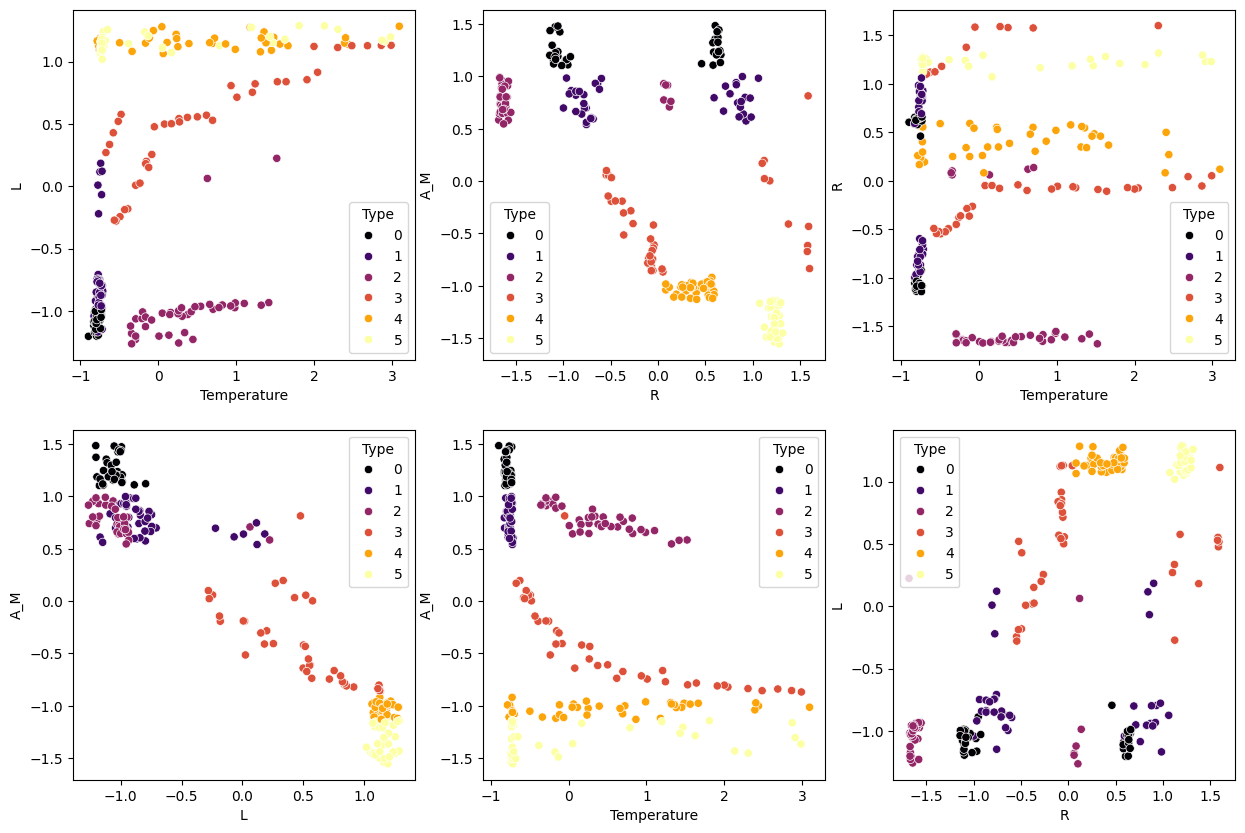
\includegraphics[width=1\linewidth]{figures/Manual.png}
\end{figure}

Vemos aqui que os \textit{clusters} são muito bem separados e de clara visualização. Em comparação com os agrupamentos feitos com agrupamento Hierárquico, KMeans e DBSCAN, podemos verificar o quão parecido os \textit{clusters} são utilizando a métrica \textit{Adjusted Rand Index} (ARI).
\begin{longlisting}
    \begin{minted}{py}
        from sklearn.metrics import adjusted_rand_score

        ariHierarchical = adjusted_rand_score(dC['Type'], categoriasHier)
        ariKMeans = adjusted_rand_score(dC['Type'], categoriasKMeans)
        ariDBSCAN = adjusted_rand_score(dC['Type'], categoriasDBSCAN)
        
        print(f'ARI Hierárquico: {ariHierarchical:.3f}')
        print(f'ARI KMeans: {ariKMeans:.3f}')
        print(f'ARI DBSCAN: {ariDBSCAN:.3f}')
    \end{minted}
\end{longlisting}
\begin{verbatim}
    ARI Hierárquico: 0.396
    ARI KMeans: 0.397
    ARI DBSCAN: 0.406
\end{verbatim}

Podemos ver então que os \textit{clusters} formados pelos métodos de agrupamento hierárquico, KMeans e DBSCAN são relativamente inferiores (DBSCAN $>$ KMeans $>$ Hierárquico) quando comparados às categorias definidas manualmente, no entanto, alguns \textit{clusters} obtidos por estes métodos são relativamente parecidos com os manuais.

Um comentário importante a ser feito é em relação ao uso do \verb|random_state=2|no KMeans. Ao impormos isso, a \textit{clusterização} fica única, porém ela pode não ser a melhor formação de \textit{clusters} quando fazemos \verb|kmeans = KMeans(n_clusters=bestNumberClustersKMeans, random_state=2).fit(scaledNumdS)|, dado que existe uma variedade de \verb|random_state| que nos dão um valor ótimo de \textit{clusters} igual a 6, mas todos eles acabam por ser diferentes e o ARI do KMeans vai sempre mudar.